%=============================================================================
%  FARMING INTELLIGENCE AI - B.Tech Project Report (KTU format)
%  Vimal Jyothi Engineering College, Chemperi
%  Compile with pdfLaTeX + BibTeX (Overleaf default settings work).
%=============================================================================
\documentclass[12pt,a4paper]{report}

%---------------------------- Fonts (Times New Roman equivalent) --------------
\usepackage[T1]{fontenc}
\usepackage[utf8]{inputenc}
\usepackage{mathptmx}
\usepackage[english]{babel}

%---------------------------- Packages ---------------------------------------
\usepackage{graphicx}
\usepackage{amsmath,amsfonts}
\usepackage{float}
\usepackage{longtable}
\usepackage{multirow}
\usepackage{booktabs}
\usepackage{array}
\usepackage{setspace}
\usepackage{titlesec}
\usepackage{cite}
\usepackage{url}
\usepackage{tikz}
\usetikzlibrary{positioning,arrows.meta,shapes.geometric,fit}
\usepackage[left=3.5cm,top=3cm,right=3cm,bottom=3.5cm]{geometry}
\usepackage[
    font=normalsize,
    labelfont=bf,
    labelsep=colon,
    justification=centering
]{caption}
\usepackage[hidelinks]{hyperref}

%---------------------------- Formatting per KTU guidelines ------------------
% Body: Times 12 pt, 1.5 line spacing, justified
\onehalfspacing
\emergencystretch=2em
\setlength{\parindent}{1cm}

% Chapter title : 18 pt, bold, centred
\titleformat{\chapter}[display]
  {\normalfont\bfseries\centering}
  {\fontsize{18}{22}\selectfont\chaptertitlename\ \thechapter}
  {8pt}
  {\fontsize{18}{22}\selectfont}
\titlespacing*{\chapter}{0pt}{0pt}{20pt}

% Heading 2 : 16 pt, bold, left aligned
\titleformat{\section}
  {\normalfont\fontsize{16}{20}\bfseries\raggedright}
  {\thesection}{1em}{}
\titlespacing*{\section}{0pt}{44pt}{14pt}

% Heading 3 : 14 pt, bold, left aligned
\titleformat{\subsection}
  {\normalfont\fontsize{14}{18}\bfseries\raggedright}
  {\thesubsection}{1em}{}
\titlespacing*{\subsection}{0pt}{20pt}{8pt}

% Heading 4 : 12 pt, bold, left aligned
\titleformat{\subsubsection}
  {\normalfont\fontsize{12}{15}\bfseries\raggedright}
  {\thesubsubsection}{1em}{}
\titlespacing*{\subsubsection}{0pt}{14pt}{6pt}

% Figure title BELOW figure, table title ABOVE table
\captionsetup[table]{skip=6pt}
\captionsetup[figure]{skip=8pt}

\pagestyle{headings}

\bibliographystyle{IEEEtran}
\renewcommand{\bibname}{References}
\renewcommand{\arraystretch}{1.25}

%---------------------------- Project details ---------------------------------
\begin{document}

\gdef\title{CONTEXTDRIVE}

\gdef\dept{Computer Science and Engineering}
\gdef\degree{Bachelor of Technology}
\gdef\branch{Computer Science and Engineering}

\gdef\college{VIMAL JYOTHI ENGINEERING COLLEGE}
\gdef\collegeplace{CHEMPERI}

\gdef\studentA{Angith Vijayan Ne}
\gdef\studentAroll{VML23CS046}

\gdef\studentB{Christo Santhosh}
\gdef\studentBroll{VML23CS082}

\gdef\studentC{Sebastian Mathew Parayidathil}
\gdef\studentCroll{LVML23CS250}

\gdef\studentD{Umarsinan N}
\gdef\studentDroll{VML23CS234}

\gdef\guide{Ms. Anju Sreedharan}
\gdef\guidedes{Assistant Professor}

\gdef\projcordinatorA{Ms. Dinsha P K}
\gdef\projcordinatorAdes{Assistant Professor}

\gdef\projcordinatorB{Dr. Nithya V P}
\gdef\projcordinatorBdes{Associate Professor}

\gdef\projcordinatorC{Dr. Renji P Cheriyan}
\gdef\projcordinatorCdes{Professor}

\gdef\hod{Ms. Divya B}
\gdef\principal{Dr. Benny Joseph}

\gdef\acadyear{2026 - 27}
\gdef\month{October 2026}
\gdef\date{05-10-2026}

%=============================================================================
% FRONT MATTER
%=============================================================================

% Cover pages and certificate without page numbers
\pagenumbering{gobble}

%================================ Top cover ===================================
%\thispagestyle{empty}
%\begin{titlepage}
%\begin{center}
 % \vspace*{1.5cm}
 % {\fontsize{22}{28}\selectfont\bfseries \title\par}
  %\vspace{1.2cm}
  %{\large \textbf{PROJECT REPORT}\par}
  %\vspace{1.5cm}
  %
\includegraphics[height=4cm]{img/vjec}\par
  %\vspace{1.5cm}
  %{\large Submitted by\par}
  %\vspace{0.4cm}
  %{\large \textbf{\studentA} (\studentAroll)\par
  % \textbf{\studentB} (\studentBroll)\par
   %\textbf{\studentC} (\studentCroll)\par
   %\textbf{\studentD} (\studentDroll)\par}
  %\vspace{1cm}
  %{\large Guide: \textbf{\guide}, \guidedes\par}
  %\vfill
  %{\normalsize DEPARTMENT OF COMPUTER SCIENCE AND ENGINEERING\par}
  %{\normalsize\bfseries \college\ \collegeplace\par}
  %{\normalsize CHEMPERI P.O. - 670632, KANNUR, KERALA, INDIA\par}
  %{\normalsize\bfseries \month\par}
%\end{center}
%\end{titlepage}

%================================ Title page ==================================
\thispagestyle{empty}
\begin{titlepage}
\begin{center}
  \vspace*{1cm}
  {\fontsize{20}{26}\selectfont\bfseries \title\par}
  \vspace{0.8cm}
  {\large\itshape A Project Report\par
   submitted to\par
   the APJ Abdul Kalam Technological University\par
   in partial fulfillment of the requirements for the degree of\par}
  \vspace{0.4cm}
  {\large\bfseries \degree\par}
  \vspace{0.3cm}
  {\large\itshape by\par}
  \vspace{0.3cm}
  {\large\bfseries \studentA\ (\studentAroll)\par
   \studentB\ (\studentBroll)\par
   \studentC\ (\studentCroll)\par
   \studentD\ (\studentDroll)\par}
  \vspace{0.4cm}
  {\large\itshape under the supervision of\par}
  \vspace{0.2cm}
  {\large\bfseries \guide\par}
  {\large \guidedes\par}
  \vspace{1.2cm}
  
\includegraphics[height=3.5cm]{img/vjec}\par
  \vspace{0.8cm}
  {\small DEPARTMENT OF COMPUTER SCIENCE AND ENGINEERING\par}
  {\small\bfseries \college\ \collegeplace\par}
  {\small CHEMPERI P.O. - 670632, KANNUR, KERALA, INDIA\par}
  {\small\bfseries \month\par}
\end{center}
\end{titlepage}

%================================ Certificate =================================
\newpage
\thispagestyle{empty}

\begin{center}
    
\includegraphics[scale=.60]{img/vjec_header}\par
    \vspace{2pt}
    \normalsize\textbf{DEPT. OF COMPUTER SCIENCE AND ENGINEERING}

    \vspace{3pt}
    \large\textbf{CERTIFICATE}
\end{center}

\vspace{0.2cm}

\noindent
\small
This is to certify that the report entitled \textbf{\title} submitted by\\
\textbf{\studentA} (\studentAroll), \textbf{\studentB} (\studentBroll),
\textbf{\studentC} (\studentCroll) \& \textbf{\studentD} (\studentDroll)
to the APJ Abdul Kalam Technological University in partial fulfillment of
the B.Tech.\ degree in \branch\ is a bonafide record of the project work
carried out by them under our guidance and supervision. This report in any
form has not been submitted to any other University or Institute for any
purpose.

\vspace{0.3cm}

\begin{singlespace}
\small
\noindent
\begin{tabular}{@{}p{7.2cm} p{0.3cm} p{6.5cm}@{}}
\textbf{PROJECT COORDINATORS} && \textbf{PROJECT GUIDE}\\[14pt]

\textbf{\projcordinatorA} && \textbf{\guide}\\
\projcordinatorAdes && \guidedes\\
Computer Science \& Engineering && Computer Science \& Engineering\\
Vimal Jyothi Engineering College && Vimal Jyothi Engineering College\\[14pt]

\textbf{\projcordinatorB} && \\
\projcordinatorBdes && \\
Computer Science \& Engineering && \\
Vimal Jyothi Engineering College && \\[14pt]

\textbf{\projcordinatorC} && \\
\projcordinatorCdes && \\
Computer Science \& Engineering && \\
Vimal Jyothi Engineering College && 
\end{tabular}

\vspace{0.4cm}

\noindent
\begin{tabular}{@{}p{7.0cm} p{0.2cm} p{6.8cm}@{}}
Place : Chemperi & & \textbf{Head of the Department}\\[18pt]
Date : \date & & \\[8pt]
\multicolumn{3}{c}{(Office Seal)}
\end{tabular}
\end{singlespace}

% Start Roman page numbering
\pagenumbering{roman}

% Declaration
%================================ Declaration =================================
\newpage
\thispagestyle{plain}
\begin{center}
  \vspace*{30pt}
  {\fontsize{18}{22}\selectfont\textbf{DECLARATION}}\par
\end{center}
\vspace{10pt}

We hereby declare that the project report \textbf{\title}, submitted for partial fulfillment of the requirements for the award of degree of Bachelor of Technology of the APJ Abdul Kalam Technological University, Kerala is a bona fide work done by us under the supervision of \textbf{\guide}.

This submission represents our ideas in our own words and where ideas or words of others have been included, we have adequately and accurately cited and referenced the original sources.

We also declare that we have adhered to the ethics of academic honesty and integrity and have not misrepresented or fabricated any data, idea, fact or source in our submission. We understand that any violation of the above will be a cause for disciplinary action by the institute and/or the University and can also evoke penal action from the sources which have thus not been properly cited or from whom proper permission has not been obtained. This report has not previously formed the basis for the award of any degree, diploma or similar title of any other University.

\begin{singlespace}
\vspace{1.5cm}
\noindent\begin{minipage}{0.45\linewidth}
  \raggedright
  \collegeplace\\
  \date
\end{minipage}
\hfill
\begin{minipage}{0.45\linewidth}
  \raggedleft
  \textbf{\studentA}\\
  \textbf{\studentB}\\
  \textbf{\studentC}\\
  \textbf{\studentD}
\end{minipage}
\end{singlespace}


% Acknowledgement
%================================ Acknowledgement =============================
\newpage
\thispagestyle{plain}
\begin{center}
  \vspace*{30pt}
  {\fontsize{18}{22}\selectfont\textbf{ACKNOWLEDGEMENT}}\par
\end{center}
\vspace{10pt}

We are extremely grateful to \textbf{\principal}, Principal, and \textbf{\hod}, Head of the Department of Computer Science and Engineering, Vimal Jyothi Engineering College, Chemperi, for providing the facilities and resources required for the successful completion of our project.

We are highly indebted to our project guide, \textbf{\guide}, \guidedes, Department of Computer Science and Engineering, for her valuable guidance, constant supervision and encouragement throughout the work. Her suggestions helped us to shape the idea of a smartphone-based context-aware driver assistance system into a well defined project.

We express our sincere thanks to our project coordinators, \textbf{\projcordinatorA} and \textbf{\projcordinatorB}, and to all the faculty members of the department for the support and co-ordination extended to us in bringing out this project in time. Our thanks and appreciation also go to the authors of the research papers and other literature that we have referred to in this project.

Last but not the least, we would like to express our gratitude to our parents and friends for their kind cooperation and encouragement.

\vspace*{20pt}
\begin{flushright}
  \textbf{\studentA}\\
  \textbf{\studentB}\\
  \textbf{\studentC}\\
  \textbf{\studentD}
\end{flushright}


% Abstract
%================================ Abstract ====================================
\chapter*{Abstract}
\addcontentsline{toc}{chapter}{Abstract}

Road safety is significantly affected by a combination of factors, including driver inattention, adverse weather conditions, vehicle speed, and complex traffic environments. This project, \textbf{ContextDrive}, presents a smartphone-based, context-aware driver assistance system designed to improve road safety by assessing driving risk in real time.

The system utilizes a standard smartphone equipped with a rear camera, GPS receiver, and internet connectivity to gather comprehensive driving data. It integrates real-time camera frames for object detection, GPS data for speed and location analysis, weather information via the OpenWeatherMap API, and time-based context. A lightweight object detection model, YOLOv8 Nano (YOLOv8n) running on Google LiteRT (formerly TensorFlow Lite), identifies vehicles and obstacles, while an intelligent engine analyzes these multiple driving factors together rather than treating individual hazards independently.

To ensure transparency and build driver trust, ContextDrive provides transparent safety recommendations based on the combined contextual data. The system continuously estimates the current driving risk score and delivers timely alerts to the driver. The proposed architecture performs entirely on-device, ensuring real-time responsiveness and privacy without the need for expensive or specialized external hardware.

By combining computer vision, edge computing, and context-aware risk analysis, the platform provides drivers with an affordable, portable, and practical solution. ContextDrive enhances situational awareness, promotes safer driving habits, and offers an intelligent approach to proactive accident prevention.

%=============================================================================
% TABLE OF CONTENTS
%=============================================================================

\singlespacing

\tableofcontents
\clearpage

%=============================================================================
% LIST OF FIGURES
%=============================================================================

\listoffigures
\phantomsection
\addcontentsline{toc}{chapter}{List of Figures}
\clearpage


%=============================================================================
% LIST OF ABBREVIATIONS
%=============================================================================

%=========================== List of abbreviations ============================
\chapter*{List of Abbreviations}
\addcontentsline{toc}{chapter}{List of Abbreviations}
\begin{singlespace}
\begin{longtable}{p{3cm} p{10.3cm}}

\textbf{ADAS} & Advanced Driver Assistance Systems\\[3pt]
\textbf{AI} & Artificial Intelligence\\[3pt]
\textbf{API} & Application Programming Interface\\[3pt]
\textbf{CNN} & Convolutional Neural Network\\[3pt]
\textbf{DFD} & Data Flow Diagram\\[3pt]
\textbf{ER} & Entity Relationship\\[3pt]
\textbf{GPS} & Global Positioning System\\[3pt]
\textbf{JSON} & JavaScript Object Notation\\[3pt]
\textbf{LBS} & Location-Based Services\\[3pt]
\textbf{ML} & Machine Learning\\[3pt]
\textbf{UI} & User Interface\\[3pt]
\textbf{YOLO} & You Only Look Once\\

\end{longtable}
\end{singlespace}

% Return to 1.5 line spacing for the main report
\onehalfspacing

%=============================================================================
% MAIN BODY
%=============================================================================

\cleardoublepage
\setcounter{page}{1}
\pagenumbering{arabic}

\chapter{Introduction}

\section{Overview}

Road safety depends on several important factors such as vehicle speed, weather conditions, visibility, traffic density, and driver attention. Drivers often make decisions based on personal experience, traditional practices, or limited observations of their immediate surroundings. This can make safe driving difficult, especially when environmental and traffic conditions change rapidly.

ContextDrive is a smartphone-based context-aware driver assistance system developed to help drivers make safer driving decisions using sensor data and Artificial Intelligence. The system combines computer vision, global positioning systems (GPS), weather intelligence, and transparent decision logic in a single platform.

The system uses a standard smartphone equipped with a rear camera to collect important visual parameters such as nearby vehicles and obstacles. GPS information is also considered for analyzing the current speed and location. A machine learning model uses these inputs to detect road users and estimate the distance to potential hazards.

In addition to object detection, the system provides contextual risk assessment and safety guidance based on the available telemetry and environmental information. A transparent rule-based engine helps the user understand the factors influencing the current risk level. Weather intelligence provides real-time rain and visibility-related information to support better situational awareness.

The system also includes a multi-dimensional context vector that continuously updates the driving risk state. An intuitive and responsive interface makes the platform easy to use directly from a dashboard-mounted mobile device.

\section{General Background}

Modern driving can benefit from technologies that provide accurate and timely information about road conditions. Smartphone sensors allow vehicle telemetry and visual data to be collected directly from the dashboard. In this system, the smartphone camera and GPS receiver gather live readings and make the information available to the application.

Machine learning can be used to analyze visual and environmental parameters and identify potential hazards on the road. This helps reduce dependence on manual risk estimation by the driver. Explicit reasoning further improves the system by showing the important factors that influence a safety recommendation, ensuring the driver understands why a warning was issued.

Weather conditions also have an important role in driving safety. Visibility, rainfall, and time of day can severely affect braking distance and reaction times. Therefore, the system combines visual, telemetry, and weather information to provide more useful and context-aware driving guidance.

Contextual interactions are also considered because driving risk depends not only on a single hazard but also on how multiple factors combine. The risk engine provides a comprehensive assessment by evaluating speed, proximity, and environment together. Thus, the system brings different driving information sources together in one cohesive platform.

\section{Problem Statement}

Drivers need to make important split-second decisions regarding speed, following distance, and maneuvering. However, the required information is often available through different and disconnected sources or is difficult to perceive manually. Drivers may have to separately judge traffic distance, monitor their speed, and mentally adjust for weather or visibility conditions.

Many existing driver assistance systems mainly focus on detecting a specific hazard in isolation, such as a forward collision or lane departure. Such systems may not provide integrated contextual monitoring, transparent explanations for their warnings, or live environmental adjustments in the same affordable platform. Access to reliable, multi-factor safety information can also be difficult for users who do not own vehicles with expensive, built-in advanced driver assistance systems (ADAS).

\section{Scope of the System}

The ContextDrive system covers several major areas of driver assistance and safety monitoring. It provides real-time object detection using a smartphone camera, GPS-based telemetry insights, weather-aware risk adjustments, and time-based contextual analysis. The system also includes explicit reasoning logic for understanding risk predictions and a multi-dimensional context vector for analyzing combined driving factors. A responsive dashboard interface allows drivers to access these features directly from a mounted mobile device.

The system also provides on-device data processing for ensuring privacy and low-latency performance without requiring specialized external hardware. It is intended to support drivers in maintaining situational awareness and making safer decisions rather than replacing their attention or active vehicle control.

\section{Objectives}

\begin{itemize}
    \item To develop a smartphone based context-aware driver assistance system for real time driving risk assessment.
    \item To integrate camera, GPS, weather, and time based information for comprehensive driving context analysis.
    \item To generate a risk score and provide timely, transparent safety recommendations.
    \item To improve driver awareness and promote safer driving without requiring additional hardware.
\end{itemize}
\chapter{Literature Review}

\section{Personalised Driver Risk Assessment with Adaptive Feedback using Crowdsensed Telemetric Data}

The rapid evolution of Intelligent Transport Systems (ITS) has brought significant advancements in how driver behavior is monitored and evaluated. Traditional approaches often relied on expensive, proprietary in-vehicle hardware such as On-Board Diagnostics (OBD-II) dongles or dedicated inertial measurement units (IMUs). However, recent trends have shifted towards utilizing the ubiquitous presence of smartphones. This paper by Auwal Sagir Muhammad et al., published in IET Intelligent Transport Systems (IET, 2025), presents a comprehensive framework for assessing driver risk using such crowdsensed telemetric data. The study focuses on transforming raw GPS traces and temporal data into structured, actionable driving risk indicators. By avoiding complex hardware, this approach democratizes driver profiling, making it accessible to a wider population and enabling large-scale, crowdsourced data collection for traffic safety analysis.

\subsection{Methodology}
The authors utilized a vast dataset of crowdsensed telemetric data collected from standard smartphones to engineer several highly specific GPS-derived driver risk indicators. The core of their methodology involved developing algorithms to filter out GPS noise and smooth the trajectory data before analysis. From this refined data, they established specific numerical thresholds for critical driving events. For instance, harsh braking was calculated by analyzing negative acceleration thresholds over consecutive GPS points, while rapid acceleration was identified through sudden positive velocity spikes. Overspeeding was determined by continuously comparing the GPS-derived vehicle speed against mapped speed limits obtained from external routing APIs. Furthermore, the turning rate was computed by analyzing the delta in GPS bearing over time, identifying aggressive cornering. 

Crucially, the system incorporated contextual flags based on the driving environment. Nighttime driving and rainy weather conditions were used to dynamically modulate the risk thresholds, acknowledging that a safe speed in broad daylight might be inherently dangerous during a nighttime downpour. These engineered indicators provided a structured, rule-based approach for extracting interpretable driving risk features from raw telemetric data. Various machine learning models, including Support Vector Machines and Random Forests, were then applied to evaluate how these engineered indicators effectively capture driving volatility and predict overall driver risk profiles.

\subsection{Advantages}
The proposed system introduces validated feature engineering methods for transforming raw GPS, temporal, and weather information into highly meaningful driver behavior indicators. A significant advantage of this system is its inherent scalability and cost-effectiveness; by relying entirely on crowdsensed smartphone data, it eliminates the need for any specialized vehicle modifications. Furthermore, by relying on well-defined, threshold-based rules rather than opaque deep learning models for feature extraction, the approach provides an easily interpretable solution. This transparency allows the system to generate adaptive, understandable feedback for the driver, explaining exactly which behaviors (e.g., frequent harsh braking) contributed to their risk profile.

\subsection{Disadvantages}
Despite its strengths, the methodology presents notable limitations. One major limitation is that the proposed thresholds for harsh braking, acceleration, and turning were validated within a specific machine learning pipeline and a particular regional context. Driving cultures and road topologies vary drastically across the globe; therefore, these rigid numerical values may require significant recalibration when applied to different geographical driving environments. Additionally, a pure telematics approach lacks visual context. If the system detects harsh braking, it cannot determine whether the driver was driving aggressively or reacting appropriately to a child suddenly running into the street. This lack of visual situational awareness highlights the need for systems that integrate telematics with camera-based perception, a gap that the ContextDrive system aims to bridge.

\section{A New CNN Based Object Detection System for Autonomous Mobile Robots Based on Real World Vehicle Datasets}

The deployment of accurate and reliable object detection models is a cornerstone of modern autonomous navigation and advanced driver-assistance systems. While cloud-based deep learning models have achieved remarkable accuracy, they suffer from latency and require continuous internet connectivity, making them unsuitable for critical driving safety applications. This paper by Udink Aulia et al., published in Heliyon (Elsevier, 2024), addresses this challenge by presenting a lightweight object detection system specifically designed for autonomous mobile robots and edge devices. The study focuses on balancing real-time processing speeds with high detection accuracy in real-world environments, heavily utilizing transfer learning to adapt generic models to specific navigational tasks.

\subsection{Methodology}
To achieve real-time performance on hardware-constrained edge devices, the authors developed a vehicle detection system utilizing the SSD (Single Shot MultiBox Detector) framework paired with a MobileNetV2 backbone and an FPN-Lite (Feature Pyramid Network) architecture. The MobileNetV2 backbone employs depthwise separable convolutions to drastically reduce the computational complexity and parameter count compared to standard convolutional neural networks (CNNs). The FPN-Lite structure allows the model to construct high-level semantic feature maps at all scales, significantly improving the detection of small or distant vehicles, which is critical for early collision warning.

To overcome the limitations of generic pre-trained models, which often fail to generalize to specific deployment environments, the authors employed extensive transfer learning. The pre-trained detector was fine-tuned on a newly collected and meticulously annotated real-world vehicle dataset. This dataset was specifically curated to represent the lighting, weather, and traffic conditions the autonomous robots would actually face. Several training configurations, including various learning rates, batch sizes, and data augmentation techniques (such as random cropping, flipping, and color jittering), were tested. The models were then rigorously benchmarked to identify the optimal hyperparameters that maximize the mean Average Precision (mAP) while keeping inference latency low enough for real-time mobile robot navigation.

\subsection{Advantages}
The study provides compelling empirical evidence that transfer learning and fine-tuning of a lightweight SSD MobileNetV2 detector can significantly improve vehicle detection accuracy while maintaining strict real-time performance. This provides a highly practical, ready-to-deploy approach for domain-specific implementation on resource-constrained edge devices. By demonstrating that high accuracy does not necessitate massive computing power, the research paves the way for advanced perception systems to be deployed on affordable hardware, making safety technologies more accessible.

\subsection{Disadvantages}
The primary disadvantage of this approach is the phenomenon known as ``domain shift.'' The detection performance of the fine-tuned model heavily depends on the quality, size, and diversity of the fine-tuning dataset. If the autonomous robot or vehicle encounters conditions not well-represented in the training data---such as sudden heavy fog, snow, or nighttime driving in poorly lit areas---the model's accuracy degrades rapidly. Consequently, adapting the model to completely new environments requires substantial, time-consuming additional data collection and manual annotation efforts. This highlights the limitation of relying solely on a fixed visual dataset without integrating dynamic environmental context APIs to adjust system sensitivity.

\section{Using Contextual Data to Predict Risky Driving Events: A Novel Methodology from Explainable Artificial Intelligence}

Traditionally, driving risk assessment has focused heavily on isolated telematics variables, such as absolute speed or the frequency of hard braking. However, driving is an inherently contextual activity; a speed of 60 km/h might be perfectly safe on a dry highway but extremely dangerous on an icy residential street. This paper by Leandro Masello et al., published in Accident Analysis \& Prevention (Elsevier, 2023), investigates how these surrounding contextual factors fundamentally influence risky driving events. The research introduces a novel methodology based on explainable artificial intelligence (XAI) to move beyond isolated risk variables, analyzing how combined environmental and traffic contexts compound to create hazardous driving situations. By bridging the gap between raw data collection and human-understandable reasoning, this study highlights the growing need for transparency in modern intelligent transport systems.

\subsection{Methodology}
The researchers utilized large-scale, naturalistic telematics data collected from fleets of vehicles over an extended period. This comprehensive dataset included standard variables like GPS coordinates, vehicle speed, and acceleration profiles. Crucially, they augmented this telematics data with a rich array of contextual driving factors obtained from external geographical and meteorological databases. These included varying speed limits, real-time weather conditions (precipitation levels, visibility limits), traffic density metrics, road characteristics (such as urban vs. rural settings, intersection proximity, and road curvature), and temporal variables (time of day, day of week). 

They trained sophisticated supervised machine learning models, specifically tree-based ensembles like Random Forest and Gradient Boosting Machines (GBM), to predict the occurrence of risky driving events based on this multi-dimensional data. Tree-based models were chosen for their robust ability to handle non-linear relationships and heterogeneous data types without extensive preprocessing. However, to interpret the complex, non-linear interactions between these variables learned by the black-box models, they applied advanced XAI techniques, specifically SHAP (SHapley Additive exPlanations). Based on cooperative game theory, SHAP values allowed the researchers to quantify the exact marginal contribution of each individual contextual factor toward the likelihood of a risky driving event occurring. For instance, the SHAP analysis could reveal precisely how much "heavy rain" contributed to a model predicting a "high risk" event compared to "speeding." This provided a highly granular, feature-by-feature view of how risk is dynamically formed in real-time.

\subsection{Advantages}
The methodology effectively and quantitatively demonstrates that driving risk is determined by the combined, compounded influence of multiple contextual factors rather than isolated telematics variables. It provides a strong, evidence-based foundation for context-aware risk assessment. For example, the study proved that the danger of a sharp turn is exponentially increased when combined with poor visibility, a correlation that simple rule-based telematics systems often miss. 

Furthermore, the use of SHAP values transforms opaque machine learning predictions into transparent insights. This transparency is vital for the widespread adoption and psychological acceptance of driver assistance systems. By showing a driver exactly *why* a situation was classified as risky (e.g., ``High risk due to combination of moderate speed and heavy rain''), the system builds user trust and encourages active behavioral correction much more effectively than a generic, unexplained warning beep. It shifts the paradigm from a reactive warning system to a proactive, educational driving companion.

\subsection{Disadvantages}
Despite its significant contributions to explainability, the proposed methodology presents practical challenges for real-world deployment on edge devices. The system relies heavily on large-scale historical telematics data for supervised machine learning training. As a result, the models require extensive, computationally expensive retraining and recalibration when applied to completely different driving environments, varying vehicle types, or new geographical datasets where the baseline contextual risk factors might fundamentally differ.

Additionally, calculating SHAP values for complex ensemble models is incredibly resource-intensive. While this methodology is highly suitable for post-trip analysis, driver debriefing, or batch processing on powerful backend servers, running these XAI algorithms continuously in real-time on a resource-constrained edge device or consumer smartphone presents a massive computational bottleneck. For real-time applications like ContextDrive, simpler, deterministic rule-based engines or highly optimized, quantized neural networks must be employed to provide instant feedback without draining the device's battery or causing thermal throttling, even if they sacrifice some of the deep nuance provided by full SHAP analysis.
\section{Optimizing Monocular Driving Assistance for Real Time Processing on Jetson AGX Xavier}

While autonomous vehicles often rely on expensive, multi-modal sensor suites including LiDAR, radar, and stereo cameras, consumer-grade Advanced Driver Assistance Systems (ADAS) must balance performance with cost and portability. Monocular camera systems offer a highly affordable alternative but require sophisticated computer vision algorithms to extract depth and spatial awareness from a single lens. This paper by Huy-Hung Nguyen et al., published in IEEE Access (IEEE, 2024), presents a monocular camera-based ADAS optimized specifically for high-performance edge computing, aiming to perform complex road scene understanding in real time without specialized depth sensors.

\subsection{Methodology}
The authors developed a unified vision pipeline designed to simultaneously handle multiple perception tasks, such as vehicle detection, pedestrian tracking, and traffic sign recognition, using a single live monocular camera feed. The core of their methodology involved deeply optimizing these lightweight object detection models for deployment on the NVIDIA Jetson AGX Xavier, a powerful embedded edge computing platform. 

To achieve high frame rates, they integrated aggressive optimization techniques. This included tensor optimization using NVIDIA's TensorRT, which fuses network layers and optimizes memory access patterns. Furthermore, they employed reduced precision inference, converting the neural network weights from standard 32-bit floating-point (FP32) to 16-bit floating-point (FP16) or 8-bit integer (INT8) representations. This quantization drastically reduces memory bandwidth requirements and accelerates mathematical operations. The performance of these highly optimized models was then rigorously benchmarked against standard baseline architectures to meticulously evaluate the trade-offs between frame rate throughput, processing latency, and overall detection accuracy in highly dynamic driving scenarios.

\subsection{Advantages}
The research convincingly demonstrates that a single monocular camera, when paired with heavily optimized lightweight object detection algorithms, can reliably perform complex, real-time perception tasks required for driver assistance. By achieving high frame rates and low latency, the system validates the feasibility of comprehensive camera-based road scene understanding without needing specialized, expensive sensors like LiDAR. This approach significantly reduces the hardware cost and complexity of implementing ADAS features in standard vehicles.

\subsection{Disadvantages}
The primary limitation of this research lies in its hardware specificity. The system's architecture, memory management, and specific tensor optimization enhancements are heavily tailored specifically for the NVIDIA Jetson AGX Xavier hardware platform and its unique GPU architecture. While powerful, the Jetson AGX Xavier is a relatively expensive embedded system not typically found in consumer smartphones. Consequently, the deployment strategy and acceleration techniques developed in this study are not directly transferable to standard smartphone-based implementations, which rely on different neural processing units (NPUs) and frameworks like Google LiteRT (TensorFlow Lite), requiring entirely different optimization paradigms.

\section{Balancing Transparency and Control: The Impact of AI Explanation Detail on User Perception in Automated Vehicles}

As artificial intelligence takes a profoundly larger role in vehicle control and driver assistance, the human-computer interaction (HCI) aspect of these systems has emerged as a critical bottleneck for widespread public adoption. A significant, persistent barrier to the acceptance of AI-driven safety systems is the well-documented ``black box'' problem, where users do not understand the underlying mechanisms dictating why a system made a certain sudden decision. This opacity often leads to ``automation surprise,'' resulting in either a complete lack of trust and system disabling, or conversely, dangerous over-reliance. This paper by Jakob Peintner et al., published in Transportation Research Interdisciplinary Perspectives (Elsevier, 2025), rigorously investigates the psychological and behavioral effects of AI explainability on user trust and perception. The core objective of the study explores how varying levels of detail and complexity in safety explanations affect a user's cognitive experience, aiming to pinpoint the optimal balance between providing necessary transparency to build trust and preventing cognitive overload that could impair situational awareness.

\subsection{Methodology}
To safely, ethically, and consistently evaluate user reactions to critical, potentially dangerous driving events, the authors designed and conducted a comprehensive virtual reality (VR) driving study. Human participants were placed in a highly realistic, immersive simulated Level-4 highly automated vehicle environment. In this setup, the vehicle handles the vast majority of the dynamic driving tasks, placing the human participant primarily in a supervisory or passenger role. Throughout the controlled simulation, the vehicle deliberately encountered various complex, randomized traffic scenarios requiring sudden automated interventions, such as a pedestrian unexpectedly darting into the road or a lead vehicle braking abruptly.

To isolate the effect of explainability, the researchers systematically tested four distinct AI explanation levels presented via an in-cabin graphical interface during these critical interventions: ``None'' (the vehicle acts completely autonomously without providing any rationale), ``How'' (the system simply describes the physical action it is taking, e.g., ``Braking hard''), ``How \& Why'' (the system describes both the action and its underlying immediate reasoning, e.g., ``Braking hard because of a pedestrian ahead''), and finally ``Contrastive \& Counterfactual'' (the system exhaustively explains why an alternative action was inherently worse and not taken, e.g., ``Braking hard because swerving into the left lane would cause a catastrophic collision with oncoming traffic''). 

To capture a holistic view of the user experience, the researchers employed a multi-modal data collection approach. Beyond standard detailed post-scenario psychometric surveys (utilizing validated Trust in Automation scales), they continuously monitored physiological and behavioral metrics during the VR simulation. This included advanced eye-tracking to measure pupil dilation as a proxy for cognitive load and stress levels, allowing them to quantitatively evaluate the psychological toll of processing each explanation level during an emergency.

\subsection{Advantages}
The study provides robust, empirical evidence addressing a core HCI challenge in vehicle automation, shifting the discourse from anecdotal UI design to data-driven psychology. The research demonstrates clearly and quantitatively that concise ``How \& Why'' explanations offer the absolute most effective balance between system transparency and user usability. The physiological data proved that while providing no explanation severely degrades trust and spikes anxiety (due to automation surprise), providing overly complex, paragraph-style contrastive explanations drastically increases cognitive load without yielding any significant improvement in perceived safety or trust. 

This research establishes a clear, evidence-based psychological framework for designing understandable and trustworthy UI/UX for driver assistance recommendations. It validates the design philosophy that ADAS interfaces must immediately answer the user's instinctive ``Why is the car doing this?'' question concisely. This perfectly aligns with modern, context-aware systems like ContextDrive, which strive to distill complex risk calculations into immediate, digestible visual feedback (such as color-coded risk rings paired with short, specific ``Why'' and ``Advice'' strings) to build rapid user consensus.

\subsection{Disadvantages}
Despite the rigorous experimental design, the primary limitation of this study is its ecological validity regarding active driver assistance. The findings are strictly based on passenger interactions within a simulated Level-4 highly automated driving environment, where the user is essentially a passive observer with the luxury of time to process graphical notifications. 

Consequently, these results may not directly, safely generalize to real-time, manual driver assistance systems (Level 1/2) where the human user is actively controlling the vehicle's steering and pedals, and requires split-second, visceral alerts to avoid collisions. In highly dynamic, high-stakes manual driving situations, even reading a relatively concise textual ``How \& Why'' explanation on a smartphone screen might cause a critical visual distraction, drawing the driver's eyes away from the road precisely when their attention is needed most. For active real-time ADAS, explanations must be delivered through highly intuitive, non-intrusive modalities---such as specific, distinct audio tones, haptic feedback, or peripheral color changes---rather than relying primarily on explicit textual descriptions, a crucial real-world nuance that this passenger-centric VR study does not fully encompass.

\chapter{Requirement Specification}

\section{Functional Requirements}

\subsection{Object Detection}
The system shall detect vehicles and obstacles in real time using the smartphone's rear camera and a lightweight object detection model.

\subsection{Contextual Risk Assessment}
The system shall continuously calculate a driving risk score based on combined inputs such as vehicle speed, proximity to detected objects, and environmental conditions.

\subsection{Transparent Safety Recommendations}
The system shall provide clear, explicit reasoning for its risk assessments. The explanations shall help users understand the important factors influencing the current safety recommendations.

\subsection{Telemetry and GPS Analysis}
The system shall use the smartphone's GPS receiver to gather live speed, location, and bearing information. This data shall be used to evaluate driving behavior and compute telemetry-based risk indicators.

\subsection{Weather and Environmental Monitoring}
The system shall obtain current weather information using the OpenWeatherMap API. Weather information, such as rain and visibility, shall be used to adjust risk calculations dynamically.

\subsection{Real-Time Visual Feedback}
The system shall provide an intuitive dashboard interface displaying the live camera feed, current risk status, and safety alerts directly on the mounted mobile device.

\subsection{Alerts and Notifications}
The system shall issue timely, context-aware warnings to the driver regarding unsafe following distances, speed violations, and adverse weather conditions.
\section{Hardware Requirements}

\subsection{Smartphone Device}
A modern smartphone serves as the primary target platform for the application, providing the necessary computational capability, memory, and internet connectivity to run the system entirely on-device without requiring external processing hardware.

\subsection{Rear Camera}
The smartphone's rear camera is used to capture live video feeds of the road scene. The continuous stream of frames is passed to the object detection model to identify vehicles and vulnerable road users in real-time.

\subsection{GPS Receiver}
The built-in GPS receiver of the smartphone is utilized to gather real-time telemetry data. It provides continuous updates on vehicle speed, location coordinates, and bearing, which are critical for driving behavior analysis and risk assessment.

\subsection{Internet Connectivity}
A stable mobile data or Wi-Fi connection is required to retrieve real-time weather information and forecasts through external APIs, ensuring the risk assessment engine operates with up-to-date environmental context.

\section{Software Requirements}

The ContextDrive system utilizes a modern mobile application architecture. It is primarily developed using Dart, Flutter, Google LiteRT, and integrates advanced object detection models and weather services.

\subsection{Dart}
Dart is the primary programming language used for the application. It provides a robust, object-oriented framework for writing both the user interface and the underlying business logic, including the risk assessment engine and telemetry processing.

\subsection{Flutter}
Flutter is used as the cross-platform application framework to develop the user interface. It provides a modular and responsive foundation for features such as the live camera dashboard, risk status displays, and setting configurations, ensuring consistent performance.

\subsection{Google LiteRT}
Google LiteRT (formerly TensorFlow Lite) is employed as the on-device machine learning inference framework. It enables the application to execute complex object detection algorithms directly on the smartphone with low latency and high efficiency.

\subsection{YOLOv8 Nano (YOLOv8n)}
YOLOv8 Nano is the lightweight object detection model integrated into the system. It is specifically optimized for edge devices and is responsible for detecting and tracking vehicles and other obstacles in the camera's field of view in real time.

\subsection{OpenWeatherMap API}
The OpenWeatherMap API is used to fetch current weather conditions based on the user's GPS coordinates. This environmental data provides critical context, such as rain or poor visibility, which is integrated directly into the contextual risk assessment calculations.

\chapter{Proposed System and Design}

\section{Proposed System}

The proposed system is a smartphone-based platform that combines computer vision, GPS telemetry, and weather intelligence to give drivers reliable and context-aware safety assistance. The system is divided into five modules.

\begin{enumerate}
    \item \textbf{Vision and Object Detection Module:} Captures real-time road scenes using the smartphone camera and detects vehicles and obstacles using a lightweight YOLOv8 Nano model.
    \item \textbf{Telemetry and GPS Module:} Collects real-time speed, location, and bearing data from the smartphone's built-in GPS receiver to track driving behavior.
    \item \textbf{Environmental Context Module:} Retrieves live weather and visibility conditions via external APIs based on the current location.
    \item \textbf{Risk Engine and Reasoning Module:} Combines visual, telemetry, and environmental data to calculate a continuous driving risk score and provides transparent explanations for its assessment.
    \item \textbf{User Interface Module:} Displays the live camera feed, current risk status, warnings, and safety recommendations through an intuitive dashboard.
\end{enumerate}

The working of the system in brief is as follows. The driver mounts the smartphone on the dashboard and starts the application. The camera begins capturing the road ahead, while the GPS receiver continuously tracks vehicle speed and location. The environmental module simultaneously checks the local weather conditions. The risk engine processes these inputs together---evaluating the distance to detected vehicles, current speed, and weather-related visibility---to determine a driving risk score. If a hazard or unsafe condition is detected, the reasoning module generates a transparent explanation. Finally, the user interface displays the live feed alongside context-aware visual warnings and safety recommendations to assist the driver.

\section{Feasibility Study}

\subsection{Technical Feasibility}
The system uses computer vision algorithms, smartphone sensors, weather APIs, and mobile application technologies, all of which are mature and well documented. It can be developed using open source frameworks like Flutter and Google LiteRT, alongside lightweight object detection models such as YOLOv8 Nano. Since modern smartphones are equipped with high-quality cameras and GPS receivers, the integration of on-device processing without external computing hardware is technically possible. Existing research has already shown that monocular camera-based perception and telematics-based risk assessment work in practice for driver assistance.

\subsection{Operational Feasibility}
The system provides a simple and intuitive dashboard interface for drivers with different technical backgrounds. It delivers real-time risk assessment, visual warnings, and transparent safety recommendations to improve driving decisions. Since the application runs entirely on the driver's smartphone mounted on the dashboard, it requires minimal setup and integrates easily into daily driving routines. The clear, explicit reasoning provided alongside alerts ensures that the system is easily understandable and builds user trust without causing cognitive overload.

\subsection{Economic Feasibility}
The project reduces the likelihood of accidents through proactive risk assessment and timely safety warnings. The development cost is low because open source software frameworks and freely available AI models are used. Unlike traditional Advanced Driver Assistance Systems (ADAS) that require expensive, specialized vehicle hardware, this system leverages the smartphone the user already owns. The minimal cost associated with standard mobile data usage for weather APIs makes the system highly affordable. The expected improvement in driver safety and accident prevention is significantly greater than the minimal operational cost of the system.

\section{Design}
The design of the system is user centric and modular. The main design diagrams are explained below.

\subsection{Architecture Diagram}
An architecture diagram provides an overall view of the major components of a software system and the connections between them. The architecture of the ContextDrive system consists of five main layers, as shown in Figure~\ref{fig:arch}.

\begin{figure}[H]
    \centering
    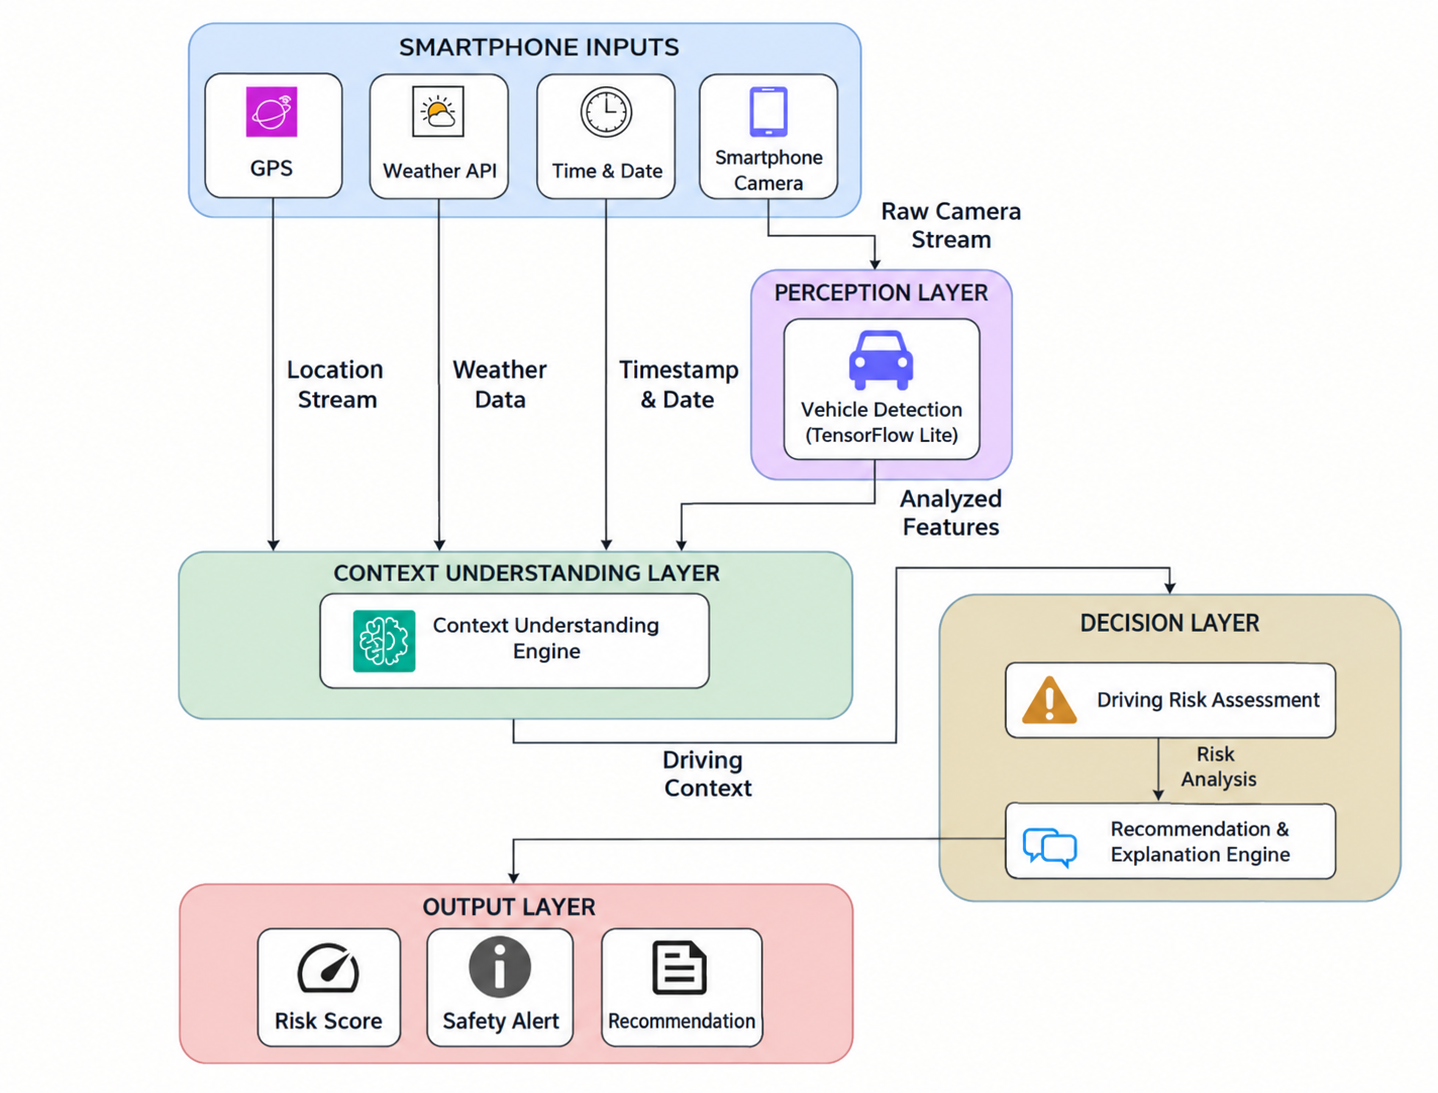
\includegraphics[width=\textwidth]{img/arch_diagram.png}
    \caption{Architecture Diagram of ContextDrive}
    \label{fig:arch}
\end{figure}

\begin{enumerate}
    \item \textbf{Input Layer:} This layer is the primary source of raw data for the system, originating from a user's smartphone. It groups several distinct data sources:
    \begin{itemize}
        \item \textit{GPS:} Outputs a location stream to the context understanding layer.
        \item \textit{Weather API:} Outputs weather data based on the current location.
        \item \textit{Time \& Date:} Outputs timestamp and date information.
        \item \textit{Smartphone Camera:} Outputs a raw camera stream to the perception layer.
    \end{itemize}
    \item \textbf{Perception Layer:} This layer processes raw sensor data from the input layer to detect environmental features. The vehicle detection engine analyzes visual data, receiving the raw camera stream and outputting analyzed features regarding detected vehicles and objects.
    \item \textbf{Context Understanding Layer:} This central layer consolidates diverse data points to create a comprehensive understanding of the current driving environment and situation. The context understanding engine builds a high-level situational model by receiving the location stream, weather data, timestamp, and analyzed features, ultimately generating a critical data stream called the driving context.
    \item \textbf{Decision Layer:} This layer analyzes the comprehensive driving context to assess risk and formulate advice in two connected stages:
    \begin{itemize}
        \item \textit{Driving Risk Assessment:} Evaluates the context data for potential hazards and risk levels, generating a risk analysis stream.
        \item \textit{Recommendation \& Explanation Engine:} Generates actionable advice and the rationale behind that advice based on the risk analysis, resulting in a consolidated assessment and recommendation stream.
    \end{itemize}
    \item \textbf{Output Layer:} This final layer presents the system’s findings and advice to the user. It receives the high-level driving context and the assessment and recommendation data. The presentation modules include the Risk Level, Safety Alert, and Recommendation.
\end{enumerate}

\subsection{Use Case Diagram}
The use case diagram illustrates the main functionalities of the ContextDrive system and the interactions of its primary actor, the driver. The driver can start a trip, view the live camera dashboard, and receive real-time driving risk assessments based on speed and proximity. The driver can also review the transparent safety explanations generated by the system to understand the factors influencing the current warnings.

\begin{figure}[H]
    \centering
    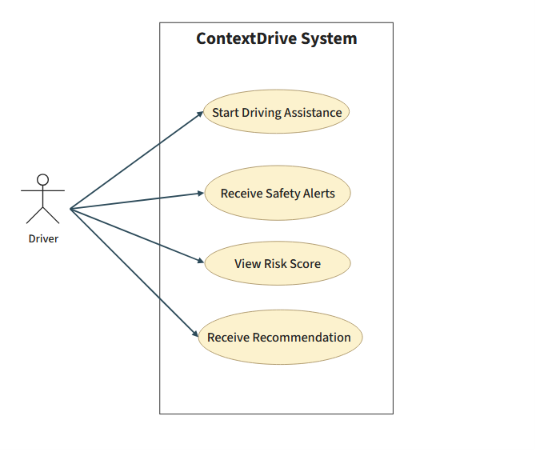
\includegraphics[width=0.8\textwidth]{img/use_case_diagram.png}
    \caption{Use Case Diagram}
    \label{fig:use_case}
\end{figure}

\subsection{Level 0 DFD}
Level 0 represents the complete ContextDrive system as a single process, as shown in Figure~\ref{fig:dfd0}. It illustrates the high-level flow of information:
\begin{itemize}
    \item \textbf{Driving Context Data (Input):} Raw environmental and sensor data (location, weather, time, camera) fed into the system.
    \item \textbf{ContextDrive (Processing):} The core engine that receives the raw data, analyzes the driving situation, and evaluates potential risks.
    \item \textbf{Risk Alerts \& Driving Recommendations (Output):} The final result generated by ContextDrive, delivering safety warnings and driving advice to the user.
\end{itemize}

\begin{figure}[H]
    \centering
    
\includegraphics[width=0.9\textwidth]{img/dfd_0.png}
    \caption{Data Flow Diagram - Level 0}
    \label{fig:dfd0}
\end{figure}

\subsection{Level 1 DFD}
Level 1 decomposes the ContextDrive system into major processes, as shown in Figure~\ref{fig:dfd1}. The flow is structured as follows:
\begin{itemize}
    \item \textbf{Inputs:} Four external data sources feed into the central system:
    \begin{itemize}
        \item \textit{Smartphone Camera:} Sends Camera Frames.
        \item \textit{Smartphone GPS:} Sends Speed / Location.
        \item \textit{Weather API:} Sends Weather Data.
        \item \textit{Smartphone Clock:} Sends Time \& Date.
    \end{itemize}
    \item \textbf{ContextDrive System:} The central processing hub that receives and combines all four input streams.
    \item \textbf{Driver:} The final recipient who receives the Risk Score, Safety Alerts, and Recommendations generated by the ContextDrive System.
\end{itemize}

\begin{figure}[H]
    \centering
    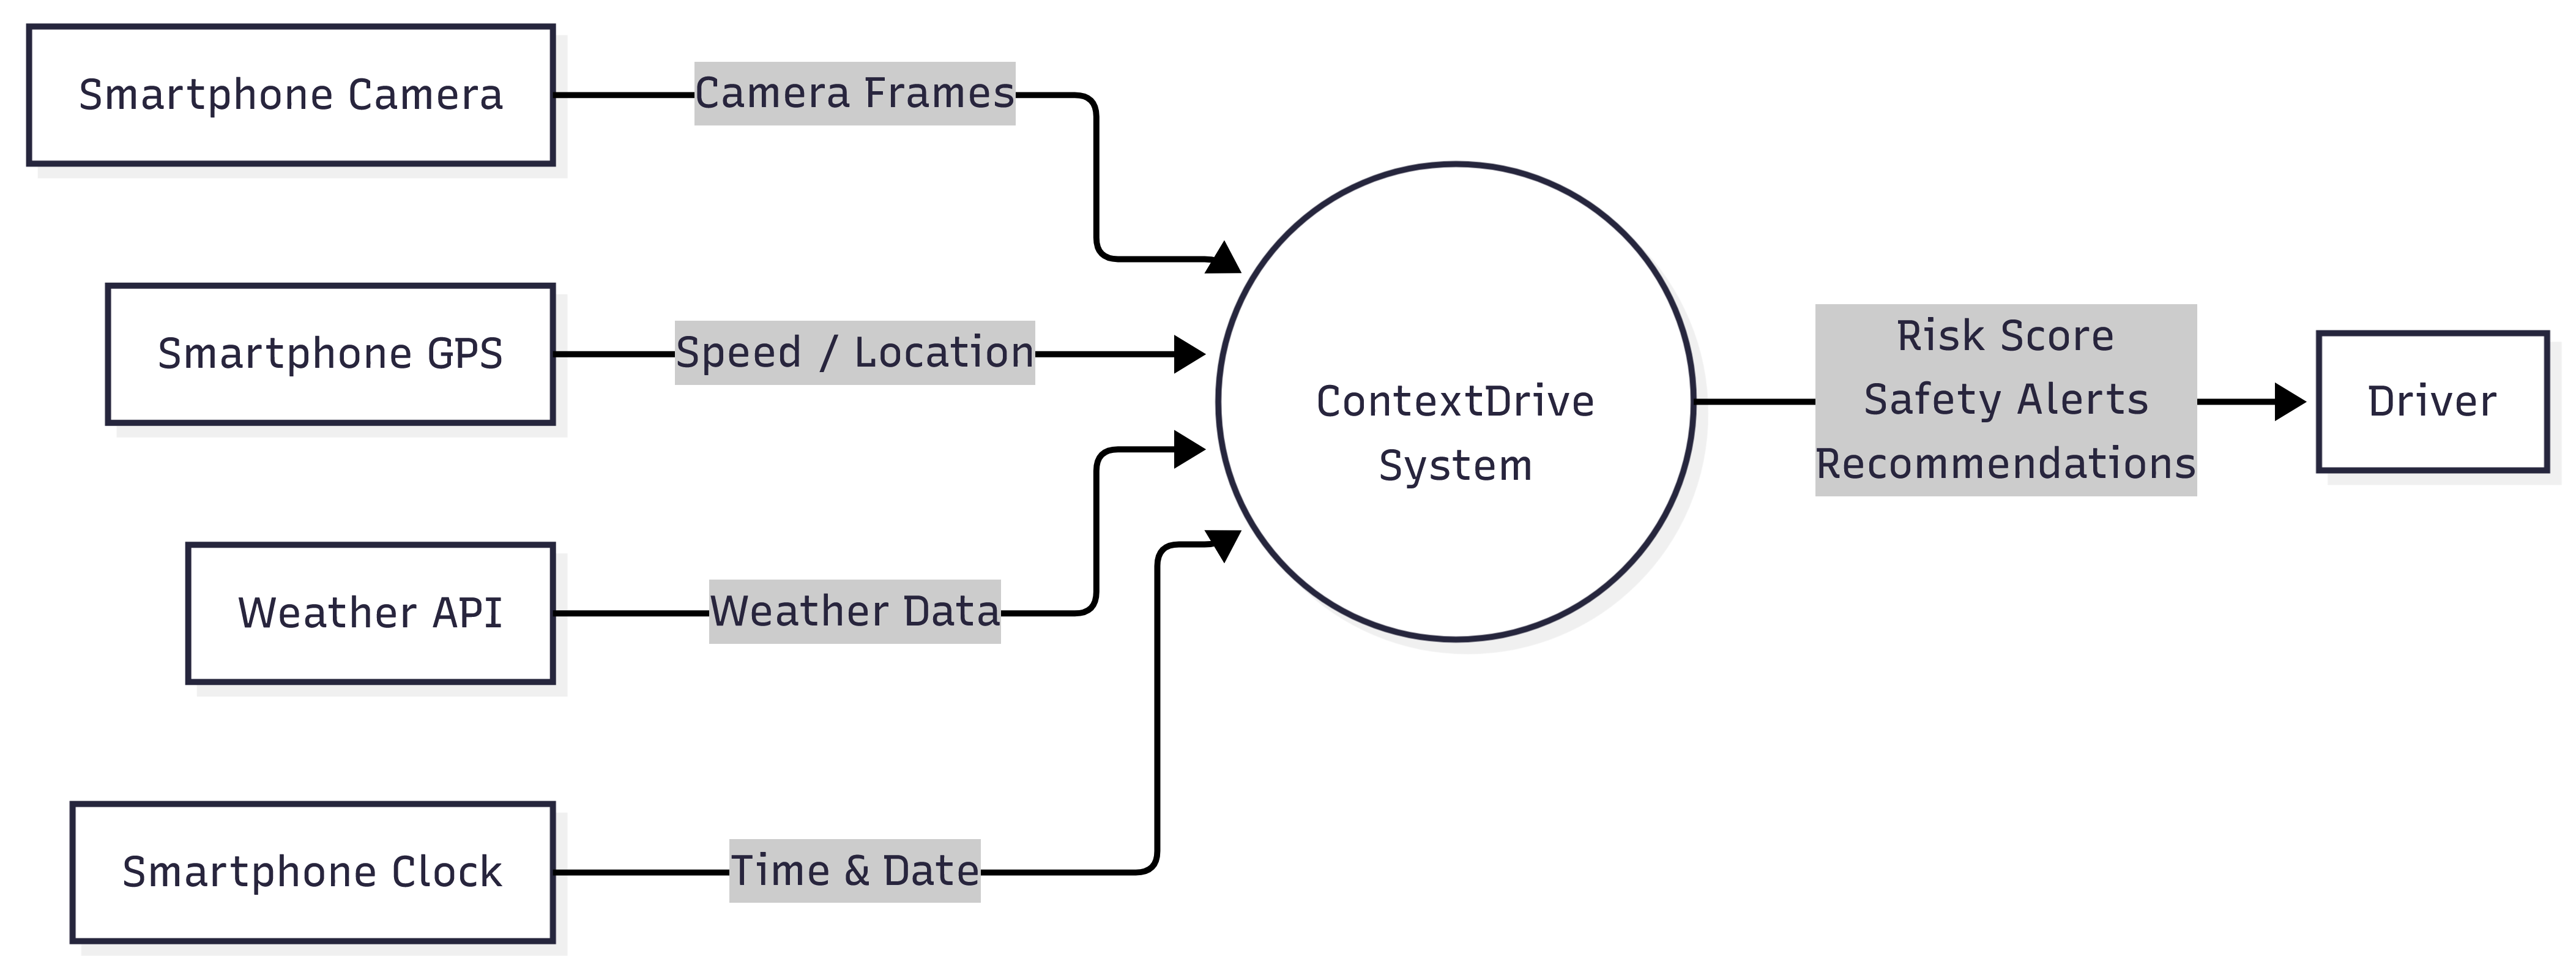
\includegraphics[width=0.9\textwidth]{img/dfd_1.png}
    \caption{Data Flow Diagram - Level 1}
    \label{fig:dfd1}
\end{figure}

\subsection{Level 2 DFD}
Level 2 DFD provides a more detailed view of the internal sub-processes within the core modules of the system, as shown in Figure~\ref{fig:dfd2}.
\begin{itemize}
    \item \textbf{Inputs:}
    \begin{itemize}
        \item \textit{Smartphone Camera:} Sends Camera Frames to the Vehicle Detection process.
        \item \textit{Smartphone GPS:} Sends Speed/Location to the Context Understanding process.
        \item \textit{Weather API:} Sends Weather Data to the Context Understanding process.
        \item \textit{Smartphone Clock:} Sends Time \& Date to the Context Understanding process.
    \end{itemize}
    \item \textbf{Processes:}
    \begin{itemize}
        \item \textit{Vehicle Detection:} Receives Camera Frames and outputs Vehicle Information to the Context Understanding process.
        \item \textit{Context Understanding:} Combines Vehicle Information, Speed/Location, Weather Data, and Time \& Date to output Driving Context to the Driving Risk Assessment process.
        \item \textit{Driving Risk Assessment:} Analyzes the Driving Context and sends a Risk Score to the Recommendation \& Explanation process.
        \item \textit{Recommendation \& Explanation:} Takes the Risk Score and sends the final Alert and Recommendation to the Driver.
    \end{itemize}
    \item \textbf{Output:}
    \begin{itemize}
        \item \textit{Driver:} The final recipient who receives the Alert and Recommendation from the Recommendation \& Explanation process.
    \end{itemize}
\end{itemize}

\begin{figure}[H]
    \centering
    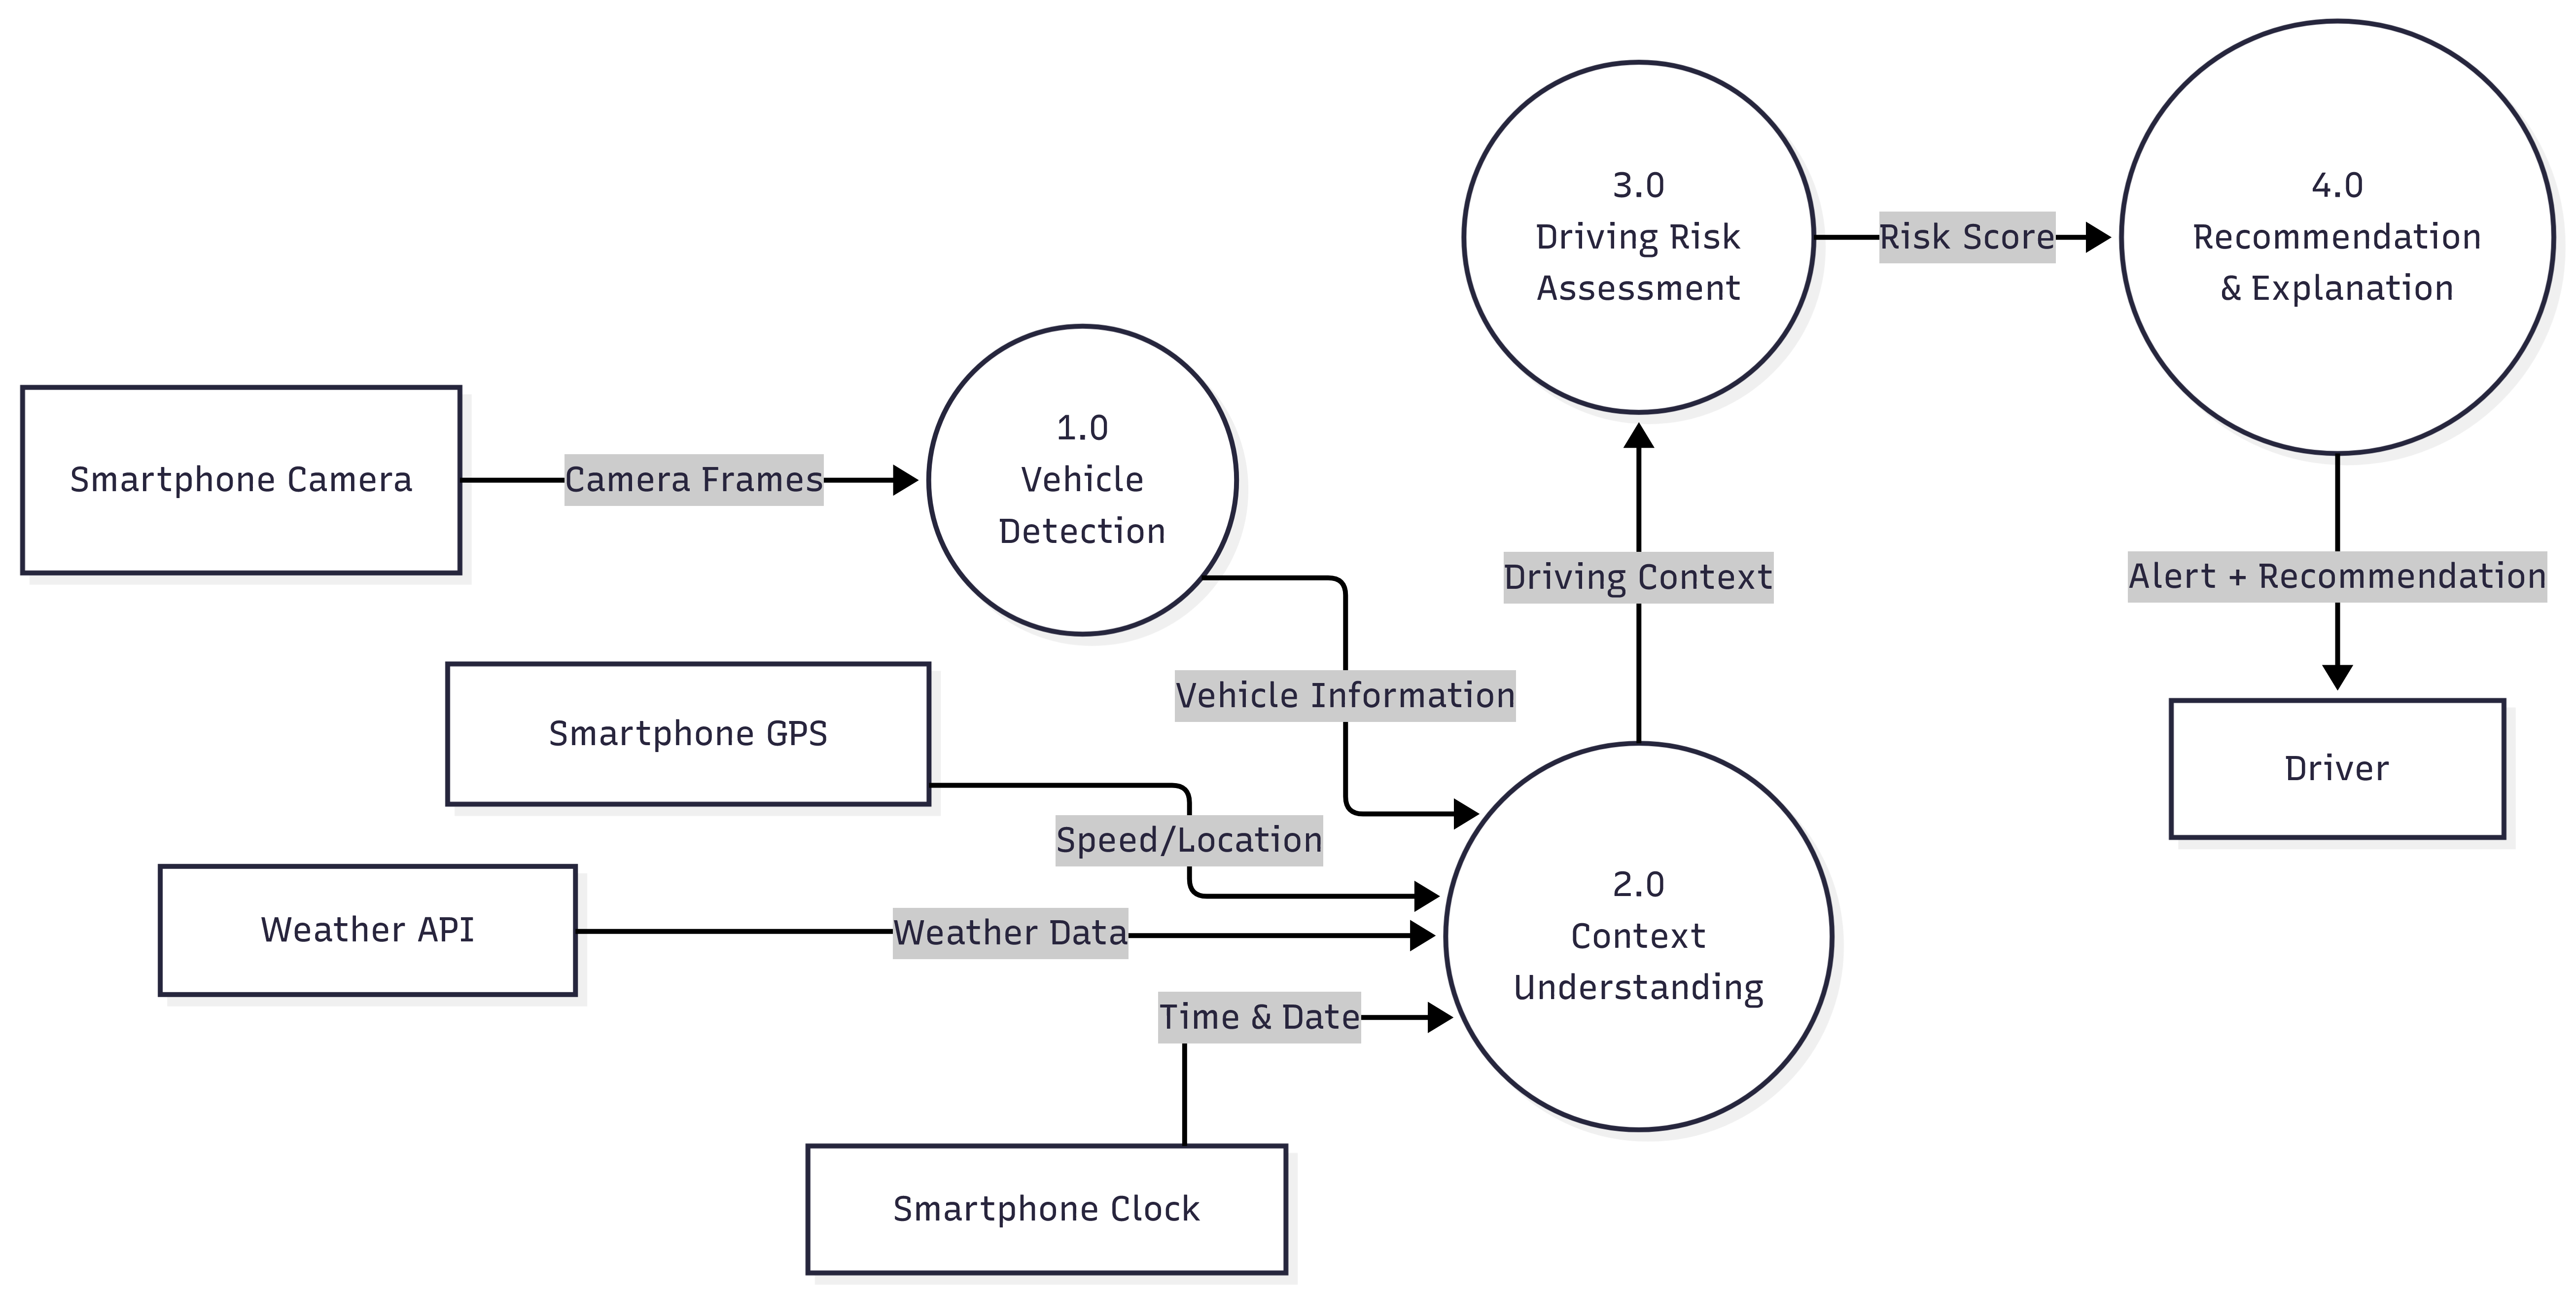
\includegraphics[width=0.9\textwidth]{img/dfd_2.png}
    \caption{Data Flow Diagram - Level 2}
    \label{fig:dfd2}
\end{figure}

\subsection{Methods and Techniques}
The ContextDrive system integrates various methods and techniques to support drivers in making informed, safe decisions. The system combines computer vision-based object detection, GPS telemetry tracking, weather data analysis, deterministic risk assessment, and transparent explainability mechanisms. These techniques work together to provide personalized and data-driven safety recommendations.

\noindent\textbf{Computer Vision-Based Object Detection}\\
The system uses the YOLOv8 Nano model via Google LiteRT to detect vehicles and obstacles in the live camera feed. This lightweight model processes camera frames efficiently on-device, providing bounding boxes and proximity estimations for critical road elements.

\vspace{0.5em}
\noindent\textbf{GPS Telemetry Tracking}\\
The system collects real-time speed, location, and bearing data from the smartphone's built-in GPS receiver. This telemetry data is used to continuously monitor the vehicle's dynamic state and movement patterns.

\vspace{0.5em}
\noindent\textbf{Weather Data Analysis}\\
Weather and visibility information is obtained using the OpenWeatherMap API based on current GPS coordinates. Parameters such as visibility distance, precipitation, and extreme weather alerts are incorporated to adjust the risk sensitivity of the system.

\vspace{0.5em}
\noindent\textbf{Deterministic Risk Assessment}\\
The system employs a rule-based deterministic risk engine to calculate a continuous driving risk score. It evaluates multiple factors, including vehicle speed, proximity to detected objects, and adverse weather conditions, to classify the driving situation into distinct risk levels.

\vspace{0.5em}
\noindent\textbf{Transparent Explainability}\\
To build trust and prevent cognitive overload, the system generates clear, explicit explanations alongside its warnings. This ensures the driver understands exactly which environmental or behavioral factors contributed to the current safety alert.

\vspace{0.5em}
\noindent\textbf{Real-Time Driver Interface}\\
The application provides a responsive Flutter-based dashboard that overlays the risk score, safety alerts, and actionable recommendations directly onto the live camera feed, ensuring seamless integration into the driving experience.
\chapter{Progress in Project}

\section{Implementation}
The ContextDrive system has been implemented as an integrated advanced driver-assistance platform combining edge-based computer vision, GPS telemetry, environmental intelligence, and deterministic risk assessment. The implementation connects these diverse modules so that real-time driving data can be processed on-device and presented to the driver through a unified, smartphone-based interface.

\subsection{Module Split-up}

\noindent\textbf{Data Acquisition and Pre-processing Module}\\
The data acquisition module collects the dynamic driving parameters required by the system. The implemented setup uses the smartphone's built-in sensors to obtain real-time video frames from the rear camera and speed, location, and bearing data from the GPS receiver. Weather information is obtained through an external weather service to provide environmental context such as visibility and precipitation. The collected values are validated and synchronized before being passed to the processing modules, ensuring that the input data is robust for risk evaluation.

\vspace{0.5em}
\noindent\textbf{Vision and Object Detection Module}\\
The vision module is responsible for identifying potential hazards on the road ahead. The implemented model uses a lightweight YOLOv8 Nano architecture optimized for mobile devices. It processes the live camera frames to detect vehicles and obstacles, generating bounding boxes and estimating proximity. The continuous object detection results are used by the risk assessment module to determine safe following distances and potential collision risks.

\vspace{0.5em}
\noindent\textbf{Environmental Context Module}\\
The environmental context module provides critical situational awareness based on the vehicle's current location. The system queries the OpenWeatherMap API to retrieve real-time weather conditions. By considering factors like fog, heavy rain, or low visibility, this module provides contextual weights that dynamically adjust the sensitivity of the risk assessment algorithms, converting raw weather data into actionable driving intelligence.

\vspace{0.5em}
\noindent\textbf{Risk Assessment Module}\\
The risk assessment module evaluates the integrated driving data to compute a continuous driving risk score. The system employs a deterministic, rule-based engine that compares vehicle speed, object proximity, and weather conditions against predefined safety thresholds. Instead of merely logging data, the module classifies the current driving situation into distinct risk levels (e.g., Safe, Warning, Critical) to facilitate immediate driver response.

\vspace{0.5em}
\noindent\textbf{Transparent Explainability Module}\\
To make the automated risk assessments easier to understand and trust, an explainability module generates explicit reasoning for its decisions. Whenever a warning or critical alert is triggered, the system analyzes the contributing factors (e.g., ``High speed in low visibility'' or ``Following too closely''). This approach ensures that the driver understands exactly why an alert was issued, reducing cognitive overload and improving the interpretability of the assistance system.

\vspace{0.5em}
\noindent\textbf{User Interface and Dashboard Module}\\
The user interface module provides a seamless and intuitive dashboard for the driver. The mobile application overlays the live camera feed with real-time bounding boxes, the current risk score, safety alerts, and transparent recommendations. It is designed to deliver critical information efficiently without distracting the driver from the road. 

\subsection{Tools and Techniques}

\noindent\textbf{Frontend Development}\\
The frontend of the system is developed using the Flutter framework with the Dart programming language. Flutter provides a highly responsive, cross-platform UI toolkit that enables the creation of a smooth, real-time camera dashboard. It handles the display of live video feeds, floating UI overlays for risk scores, and the presentation of transparent safety explanations.

\vspace{0.5em}
\noindent\textbf{Edge AI and Computer Vision}\\
The core perception capabilities are powered by Google LiteRT (formerly TensorFlow Lite), which allows the YOLOv8 Nano model to execute efficiently directly on the smartphone hardware. This edge-AI approach ensures that video frames are processed locally in real-time, eliminating network latency and preserving driver privacy since video data never leaves the device.

\vspace{0.5em}
\noindent\textbf{Telemetry and Location Services}\\
The system utilizes native smartphone GPS sensors accessed via Flutter location and geolocator packages. This provides the continuous stream of speed, heading, and coordinate data necessary for the risk engine to accurately monitor driving dynamics.

\vspace{0.5em}
\noindent\textbf{Environmental Data Services}\\
The OpenWeatherMap API is used as the external cloud service for retrieving hyper-local weather data. Standard HTTP request libraries in Dart handle the API communication, fetching relevant environmental context based on the current GPS coordinates to enhance the system's situational awareness.

\chapter{Expected Outcome}

The expected outcome of the ContextDrive project is a user-friendly, smartphone-based advanced driver-assistance system (ADAS) that assists drivers in making informed, safe decisions using real-time camera, GPS, and environmental information. The system integrates edge-based computer vision, continuous telemetry monitoring, environmental intelligence, deterministic risk assessment, and transparent explainability into a single mobile application. The vision and object detection module is expected to identify potential hazards, such as leading vehicles, by efficiently processing live camera frames on-device. The risk assessment module is expected to provide practical safety evaluations by analyzing vehicle speed, object proximity, and adverse weather conditions, helping drivers maintain safe following distances and adapt to changing environments. The transparent explainability module is expected to improve trust and interpretability by explicitly identifying the critical factors (e.g., high speed in low visibility) that triggered a safety warning. Overall, the project is expected to provide an integrated smart driving platform that supports data-driven risk evaluation, enhanced situational awareness, and context-aware safety guidance.

The system is also expected to provide a seamless and accessible interface through which drivers can view their live camera feed, real-time risk scores, bounding boxes for detected hazards, and actionable safety recommendations. By bringing these functionalities together in a single smartphone application without the need for expensive dedicated hardware, the project aims to reduce the complexity of driving safety systems and support drivers in adopting safer, more proactive driving habits.
\chapter{Conclusion}

The ContextDrive project provides an integrated advanced driver-assistance platform that combines edge-based computer vision, GPS telemetry tracking, environmental intelligence, deterministic risk assessment, and transparent explainability. By using continuous vehicle dynamics and environmental data, the system helps drivers identify potential road hazards and receive real-time, actionable safety guidance. The integration of explainable AI improves the transparency of risk assessments, while the edge-processing architecture supports privacy and rapid response times. The mobile-first approach further provides accessible safety features without requiring expensive hardware modifications. Overall, the project aims to support drivers in making informed, data-driven decisions and adopting safer, more proactive driving habits.
%=============================================================================
% APPENDICES
%=============================================================================

\appendix

% ============================================================
% APPENDIX A
% ============================================================

% \chapter{Appendix A Title}
% Content goes here.
% ============================================================
% APPENDIX B
% ============================================================

% \chapter{Appendix B Title}
% Content goes here.

%=============================================================================
% REFERENCES
%============================================================================% REFERENCES
%============================================================================% REFERENCES
%============================================================================
% REFERENCES
%=============================================================================

\singlespacing

\renewcommand{\bibname}{References}
\addcontentsline{toc}{chapter}{References}

\nocite{*}
\bibliographystyle{IEEEtran}
\bibliography{reference/refs}

\end{document}